\documentclass[tikz]{standalone}
\usepackage{xcolor, amsmath, amssymb}
\usetikzlibrary{arrows.meta}
\begin{document}
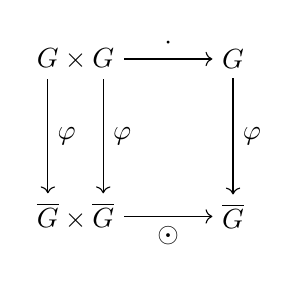
\begin{tikzpicture}[scale=2]
\node at(0,0)(gg){$G\times G$};
\node at(1,0)(g){$G$};
\node at(0,-1)(hh){$\overline G\times\overline G$};
\node at(1,-1)(h){$\overline G$};
\path[->, transform canvas={xshift=10pt}] (gg) edge node[right]{$\varphi$} (hh);
\path[->, transform canvas={xshift=-10pt}] (gg) edge node[right]{$\varphi$} (hh);
\path[->]
    (g) edge node[right]{$\varphi$} (h)
    (gg) edge node[above]{$\cdot$} (g)
    (hh) edge node[below]{$\odot$} (h);
\end{tikzpicture}
\end{document}